\section{6LoWPAN-Sensornetz}
\myContentSectionFrame[\thesection - 6]

%----------------------------------------------------------
% Section Contiki
%===============================================================================
\subsection{Contiki-OS}
%===============================================================================


\subsubsection{Anforderungen an Softwareinfrastruktur}
%-------------------------------------------------------------------------------
\begin{frame}{\insertsubsubsection}{}
	\begin{itemize}
	\item	stromsparend
	\item	speicherschonend
	\item	bereits implementierte Netzwerkprotokolle
	\item	Multitasking
	\item	intuitive Programmierumgebung
	\end{itemize}
\end{frame}
%-------------------------------------------------------------------------------

\subsubsection{Infrastrukturentscheidung}
%-------------------------------------------------------------------------------
\begin{frame}{\insertsubsubsection}{}
	\begin{columns}
	\column{.45\textwidth}
	\begin{block}{Betriebssystem}
		\begin{proconlist}
		\contra	Speicheroverhead für OS
		\pro	Multitaskingabstraktion
		\pro	stimmige Umgebung
		%\pro	zeitsparend
		\end{proconlist}
	\end{block}

	\column{.45\textwidth}
	\begin{block}{eigene Infrastruktur}
		\begin{proconlist}
		\pro	kein Speicheroverhead
		\contra	Multitasking von Hand
		\contra	inkompatible Software
		%\contra	zeitaufwändig
		\end{proconlist}
	\end{block}
	\end{columns}

	\begin{block}{Contiki}<2->
	\begin{itemize}
	\item	Multitasking auf einem Stack \(\leadsto\) speicherschonend
	\item	grundlegende IPC-Mechanismen
	\item	implementierte Netzwerkprotokolle (6LoWPAN, CoAP, \dots)
	\item	vorgesehene Schnittstelle für Sleeping Modes
	\item	bereits auf ATmega128RFA1 portiert
	\item	dynamisches nachladen von Modulen
	\end{itemize}
	\end{block}
\end{frame}
%-------------------------------------------------------------------------------

%----------------------------------------------------------
\subsection[Kommunikation]{Kommunikation im 6LoWPAN-Sensornetz}
\againframe{netzwerkaufbau}


% Verwenden des Betribssystems Contiki
% Contiki ProtokollStack zeigen

\begin{frame}{\insertsection}{Protokollstack am Beispiel von Contiki-OS}
\begin{center}
\begin{tabular}{ll}
	\toprule
	\theadhll{Layer}	& \theadhll{Protocol}	\tabularnewline
	\midrule
	Application		& CoAP REST Engine (Erbium)	\tabularnewline
	Transport		& UDP	\tabularnewline
	Network			& IPv6, RPL(Routing)	\tabularnewline
	Adaption		& 6LoWPAN	\tabularnewline
	MAC			& CSMA	\tabularnewline
	Radio Duty Cycling	& CXMAC, Lpp, ContikiMAC	\tabularnewline
	Physical		& IEEE 802.15.4	\tabularnewline
	\bottomrule
\end{tabular}
\end{center}
\end{frame}

% CoAP: 
%   - abgespecktes HTTP
%   - Definition von sogenannten Ressourcen
%   - Bei Abfrage der Ressourcen mittels GET bspw. werden in diesen Ressourcen Funktionen  
%     aufgerufen um Sensorwerte zu ermitteln um diese dann zurückzuschicken
%   - Analog dazu mittels PUT können Aktoren an den Knoten geschaltet werden.

% Transportschicht: 
%   - Verwendung von UDP um Kommunikationsaufwand gering zu halten 
%   - (kein Handshake-Protokoll wie bei TCP)

% Netzwerkschicht:
% 	- Verwendung von IPV6, 
%   - und für das Routing wird RPL verwendet: spezielles Routing Protokoll für verlustbehaftete  
%     Netze

% Adaptionsschicht:
%   - Problem: IPV6 erfordert Maximum Transmission Unit (MTU) von mind. 1280 Bytes
%              Standard 802.15.4 sieht nur Paketgröße von 127 Bytes vor
%   - 6LoWPAN: ermöglicht Fragmentierung der Pakete und die Komprimierung der IPV6/UDP Header

% MAC-Schicht & Pysikalische Schicht wird durch IEEE 802.15.4 definiert.  

%----------------------------------------------------------

\begin{frame}{\insertsection}{MAC-Schicht}
	\begin{block}<+->{Definition laut IEEE 802.15.4}
		\begin{itemize}
		\item Kollisionsvermeidung: Carrier Sense Multiple Access (CSMA)
		%\item 2 Typen von Netzknoten:
		%	\begin{itemize}
		%	\item Full Function Device (FFD)
		%	\item Reduced Function Device (RFD)
		%	\end{itemize}
		\item Übertragungsverfahren:
			\begin{itemize}
			\item Slotted Mode
			\item Unslotted Mode
			\end{itemize}
		\item Verbindungsaufbau
		\end{itemize}
	\end{block}
%\end{frame}

% Kollisionsvermeidung durch CSMA
%% 2 Typen von Netzknoten: Full Function Device 
%%                         Reduced Function Device

% Slotted Mode:
%  - Übertragung mithilfe von Beacons
%  - dabei gibt es ein PAN-Koordinator, welcher die Übertragungszeiträume aufteilt.
%  - Um etwas zu senden muss sich ein Knoten mit dem Koordinator synchronisieren

% Unslotted Mode: 
%  - Übertragung ohne Beacons
%  - vor dem prüft der Knoten ob der Kanal belegt ist und sendet seine Daten sobald er frei ist
%  - Keinerlei Verwaltungsaufwand durch den PAN-Koordinator

% Verbindungsaufbau:
%  - dabei wird definiert wie ein neuer Knoten dem Netz beitritt

%\begin{frame}{\insertsection}{MAC-Schicht}
	\begin{block}<+->{In Contiki}
		\begin{itemize}
		\item Übertragungsverfahren: Unslotted Mode
		\item Verbindungsaufbau: keine Implementierung bisher
		\item Unterteilung der MAC-Schicht in:
			\begin{itemize}
				\item MAC-Schicht: Beinhaltet nur CSMA		
				\item RDC-Schicht: Zuständig für Radio Duty Cycling
			\end{itemize}		 
		\end{itemize}
	\end{block}
\end{frame}


% RDC: Zuständig für Radio Duty Cycling, d.h wichtig für die Anforderung an unser Sensornetz 	
%      energieeffizient zu sein
%----------------------------------------------------------

\begin{frame}{\insertsection}{Radio Duty Cycling}
	\begin{figure}[h]
	\centering
	\fbox{
		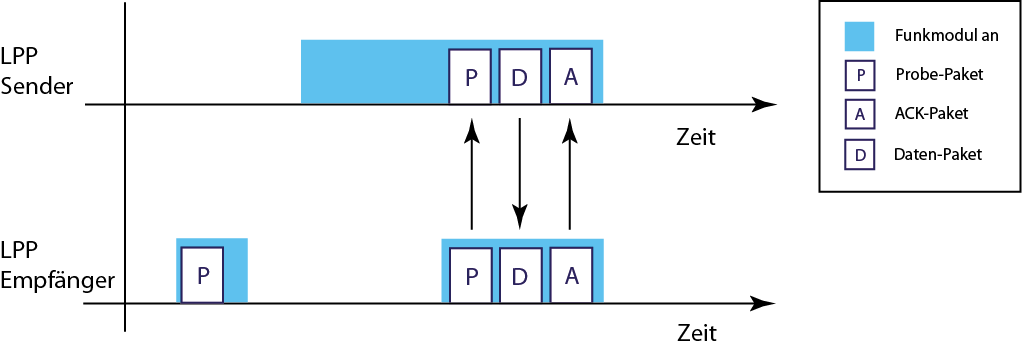
\includegraphics[scale=0.6]{pic/lpp.png}
	}
  	\caption[Lpp-Protokoll]{Lpp-Protokoll}
  	%\label{fig:dynbaum_1}
	\end{figure} 
\end{frame}

% Alle Knoten schicken Periodisch ein Probe-Paket
% Ein Knoten der etwas senden möchte, wartet auf das entsprechende Probe-Paket und sendet kurz  
%    danach sein Datenpaket
% Der Empfänger bleibt nach dem verschicken des Probe-Pakets noch kurz wach um etwaige 
%    Datenpakete zu empfangen

% Probleme: falls mehrere Sendewünsche an einen Knoten bestehen, kommt es zur Kollision


%----------------------------------------------------------
\begin{frame}{\insertsection}{Radio Duty Cycling}
	\begin{figure}[h]
	\centering
	\fbox{
		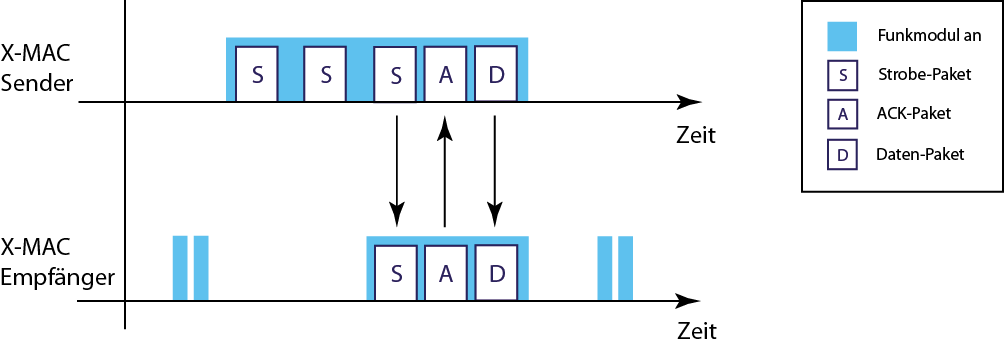
\includegraphics[scale=0.6]{pic/xmac.png}
	}
  	\caption[XMAC-Protokoll]{XMAC-Protokoll}
	\end{figure} 
\end{frame}

% Sender: sendet wiederholt Strobe-Pakete mit Addresse des Empfängers
% Empfänger: 
%    - wacht periodisch auf (man spricht von Channel Check Rate) 
%    - damit garantiert ist dass Empfänger Paket erhalten kann, müssen Strobe-Pakete mindestens 
%      solang verschickt werden, wie eine Schlafperiode beim Empänger dauert 
%    - sobald Empfänger Strobe-Paket empfängt und die Zieladresse identisch ist mit seiner 
%      Adresse, schickt er ein Acknowledgement-Paket an den Sender
%    - falls Adresse unterschiedlich ist, schläft er weiter
% Sender empfängt das Ack-Paket und sendet kurz darauf das eigentliche Datenpaket

% Nachteile:
%  - Minimal erhöhter Energieverbrauch beim Sender, da dieser in kurzer Folge mehrere 
%    Strobepakete verschicken muss


%----------------------------------------------------------

\begin{frame}{\insertsection}{Energieverbrauch am Beispiel des ATmega128RFA1}
	\begin{figure}[h]
	\centering
	\fbox{
		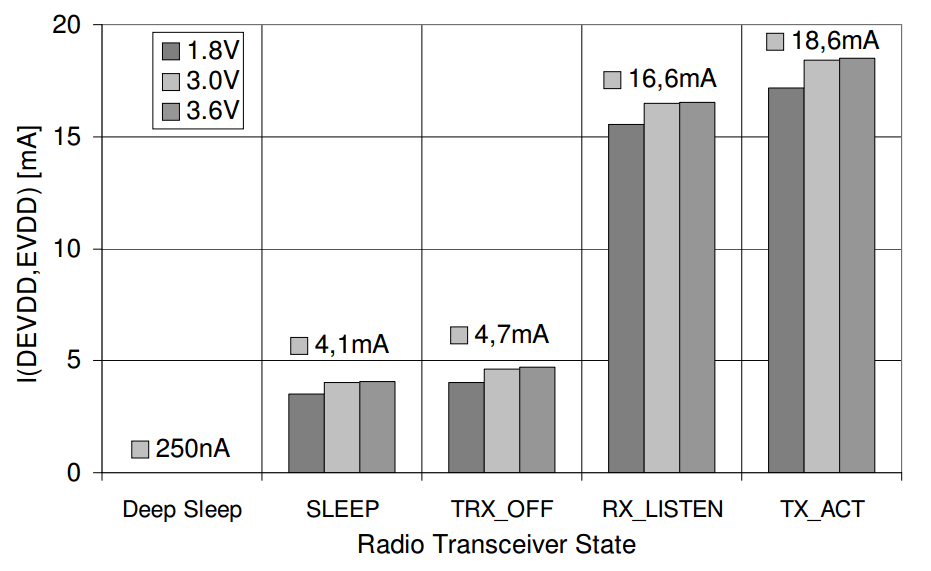
\includegraphics[scale=0.4]{pic/Verbrauch.png}
	}
  	\caption[t]{Energieverbrauch des ATmega128RFA1}
	\end{figure} 
\end{frame}

%----------------------------------------------------------


\begin{frame}{\insertsection}{Energieverbrauch am Beispiel des ATmega128RFA1}
\centering
\begin{center}
\begin{tabular}{lrrD{,}{,}{1}D{,}{,}{1}}
	\toprule
	& & & \multicolumn{2}{c}{\theadhll{Lebenszeit [Tage]}}	\tabularnewline
	\cmidrule(l){4-5}
	  \theadhll{Modus}
	  & \theadhll{Duty Cycle  [\%]}
	  & \multicolumn{1}{c}{{\theadhll{Verbrauch [\micro A]}}}
	  & \multicolumn{1}{c}{{\theadhll{800 mAh}}}
	  & \multicolumn{1}{c}{{\theadhll{2600 mAh}}}	\tabularnewline
	\midrule
	Deep Sleep 	& - 	& 0,25	& 133300	& 433300 \tabularnewline
	Sleep		& -		& 4100	& 8,1	& 26,4 \tabularnewline
	TRX ON		& 100	& 18600	& 1,8	& 5,8 \tabularnewline
	CXMAC		& 5		& 5300	& 6,3	& 20,4 \tabularnewline
				& 10	& 6000	& 5,6	& 18,1 \tabularnewline
				& 50	& 11300	& 2,9	& 9,6 \tabularnewline
	\bottomrule
\end{tabular}
\end{center}

\tiny{Hinweis: Diese Tabelle ist lediglich eine Schätzung des Energieverbrauchs,
um zu demonstrieren, wie wichtig die Senkung des Energieverbrauchs ist.
Bei Schätzung der Lebenszeiten bei Verwendung von CXMAC wurde angenommen,
dass der Mikrocontroller nur in den Sleep Modus geht.
Man kann erkennen, dass der Duty Cycle so klein wie möglich gehalten werden sollte.
Auch sollte der Deep Sleep Modus so oft wie möglich genutzt werden.}

\end{frame}

%----------------------------------------------------------



